\begin{frame}
\frametitle{Espace d'approximation / Élément de référence}
\vfill
\begin{columns}[c]
\column{.5\textwidth}
\begin{itemize}
\item Choix des hexaèdres ;
\item Cube unité, noté $\HexaRef = \ItvCC{0}{1}^{3}$ ;
\item Faces notées $(\QuadRef_f)_{f \in \Range{0}{5}}$ ;
\item Permet de se ramener à un espace identique pour chaque maille ;
\item Passage des tétraèdres aux hexaèdres :
\end{itemize}
\vfill
\begin{figure}
\centering
		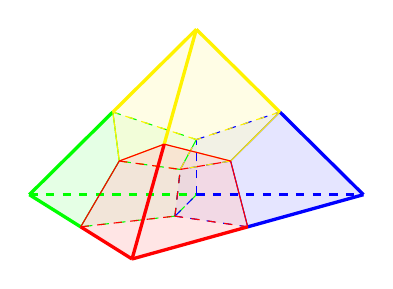
\begin{tikzpicture}[scale=3,rotate around x=270,rotate around z=45]
		%\draw[very thick] (0,0,0) -- (1,0,0) -- (0.5,0.5,0.7) -- (0,1,0) -- cycle;
		%\draw[very thick] (0,0,0) -- (0.5,0.5,0.7);
		%\draw[dashed,very thick] (1,0,0) -- (0,1,0);
		
		\fill[green!20,opacity=0.5] (0,1,0) -- (0,0.5,0) -- (0.3333,0.3333,0) -- (0.5,0.5,0) -- (0.5,0.5,0.2333) -- (0.25,0.75,0.35) -- cycle;
		
		\fill[blue!20,opacity=0.5] (1,0,0) -- (0.5,0,0) -- (0.3333,0.3333,0) -- (0.375,0.375,0.175) -- (0.5,0.5,0.2333) -- (0.75,0.25,0.35) -- cycle;
		
		\fill[yellow!20,opacity=0.5] (0.5,0.5,0.7) -- (0.75,0.25,0.35) -- (0.5,0.1666,0.2333) -- (0.375,0.375,0.175) -- (0.1666,0.5,0.2333) -- (0.25,0.75,0.35) -- cycle;

		\fill[red!20,opacity=0.5] (0,0,0) -- (0,0.5,0) -- (0.1666,0.5,0.2333) -- (0.25,0.25,0.35) -- (0.5,0.1666,0.2333) -- (0.5,0,0) -- cycle;
		
		\draw[green,dashed,very thick] (0,1,0) -- (0.5,0.5,0);
		\draw[green,dashed] (0.5,0.5,0) -- (0.3333,0.3333,0);
		\draw[green,dashed] (0.3333,0.3333,0) -- (0,0.5,0);
		\draw[green,very thick] (0,0.5,0) -- (0,1,0);
		\draw[green,dashed] (0.25,0.75,0.35) -- (0.5,0.5,0.2333);
		\draw[green,dashed] (0.5,0.5,0.2333) -- (0.375,0.375,0.175);
		\draw[green,dashed] (0.375,0.375,0.175) -- (0.1666,0.5,0.2333);
		\draw[green] (0.1666,0.5,0.2333) -- (0.25,0.75,0.35);
		\draw[green,very thick] (0,1,0) -- (0.25,0.75,0.35);
		\draw[green,dashed] (0.5,0.5,0) -- (0.5,0.5,0.2333);
		\draw[green,dashed] (0.3333,0.3333,0) -- (0.375,0.375,0.175);
		\draw[green] (0,0.5,0) -- (0.1666,0.5,0.2333);
		
		\draw[blue,very thick] (1,0,0) -- (0.5,0,0);
		\draw[blue,dashed] (0.5,0,0) -- (0.3333,0.3333,0);
		\draw[blue,dashed] (0.3333,0.3333,0) -- (0.5,0.5,0);
		\draw[blue,dashed,very thick] (0.5,0.5,0) -- (1,0,0);
		\draw[blue] (0.75,0.25,0.35) -- (0.5,0.1666,0.2333);
		\draw[blue,dashed] (0.5,0.1666,0.2333) -- (0.375,0.375,0.175);
		\draw[blue,dashed] (0.375,0.375,0.175) -- (0.5,0.5,0.2333);
		\draw[blue,dashed] (0.5,0.5,0.2333) -- (0.75,0.25,0.35);
		\draw[blue,very thick] (1,0,0) -- (0.75,0.25,0.35);
		\draw[blue] (0.5,0,0) -- (0.5,0.1666,0.2333);
		\draw[blue,dashed] (0.3333,0.3333,0) -- (0.375,0.375,0.175);
		\draw[blue,dashed] (0.5,0.5,0) -- (0.5,0.5,0.2333);
		
		\draw[yellow,very thick] (0.5,0.5,0.7) -- (0.25,0.25,0.35);
		\draw[yellow] (0.25,0.25,0.35) -- (0.5,0.1666,0.2333);
		\draw[yellow] (0.5,0.1666,0.2333) -- (0.75,0.25,0.35);
		\draw[yellow,very thick] (0.75,0.25,0.35) -- (0.5,0.5,0.7);
		\draw[yellow] (0.25,0.75,0.35) -- (0.1666,0.5,0.2333);
		\draw[yellow,dashed] (0.1666,0.5,0.2333) -- (0.375,0.375,0.175);
		\draw[yellow,dashed] (0.375,0.375,0.175) -- (0.5,0.5,0.2333);
		\draw[yellow,dashed] (0.5,0.5,0.2333) -- (0.25,0.75,0.35);
		\draw[yellow,very thick] (0.5,0.5,0.7) -- (0.25,0.75,0.35);
		\draw[yellow] (0.25,0.25,0.35) -- (0.1666,0.5,0.2333);
		\draw[yellow,dashed] (0.5,0.1666,0.2333) -- (0.375,0.375,0.175);
		\draw[yellow,dashed] (0.75,0.25,0.35) -- (0.5,0.5,0.2333);

		\draw[red,very thick] (0,0,0) -- (0,0.5,0);
		\draw[red,dashed] (0,0.5,0) -- (0.3333,0.3333,0);
		\draw[red,dashed] (0.3333,0.3333,0) -- (0.5,0,0);
		\draw[red,very thick] (0.5,0,0) -- (0,0,0);
		\draw[red] (0.25,0.25,0.35) -- (0.1666,0.5,0.2333);
		\draw[red,dashed] (0.1666,0.5,0.2333) -- (0.375,0.375,0.175);
		\draw[red,dashed] (0.375,0.375,0.175) -- (0.5,0.1666,0.2333);
		\draw[red] (0.5,0.1666,0.2333) -- (0.25,0.25,0.35);
		\draw[red,very thick] (0,0,0) -- (0.25,0.25,0.35);
		\draw[red] (0,0.5,0) -- (0.1666,0.5,0.2333);
		\draw[red,dashed] (0.3333,0.3333,0) -- (0.375,0.375,0.175);
		\draw[red] (0.5,0,0) -- (0.5,0.1666,0.2333);
		
		% centre : (0.375,0.375,0.175)
		% face 1 : (0.3333,0.3333,0)
		% face 2 : (0.5,0.1666,0.2333)
		% face 3 : (0.5,0.5,0.2333)
		% face 4 : (0.1666,0.5,0.2333)
		% edge 1 : (0.5,0,0)
		% edge 2 : (0.5,0.5,0)
		% edge 3 : (0,0.5,0)
		% edge 4 : (0.25,0.25,0.35)
		% edge 5 : (0.75,0.25,0.35)
		% edge 6 : (0.25,0.75,0.35)
		
		
		
		%\draw[very thick] (0,0,0) -- (1,0,0) -- (0,1,0) -- cycle;
		%\draw[blue] (0,0,0) -- (0.5,0.5,0.7);
		%\draw[red] (1,0,0) -- (0.5,0.5,0.7);
		%\draw[green] (0,1,0) -- (0.5,0.5,0.7);
		\end{tikzpicture}
\end{figure}
\column{.5\textwidth}
\begin{figure}
\centering
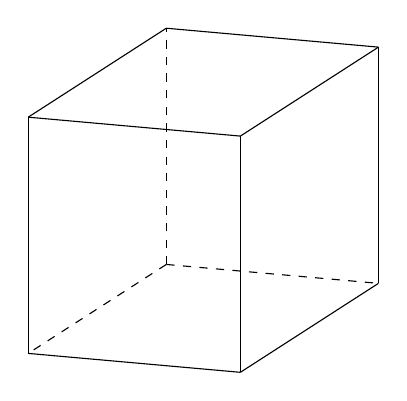
\begin{tikzpicture}[scale=3,rotate around x=270,rotate around z=258]
	% cube arriere
	\draw [dashed] (0,0,0) -- (1,0,0);
	\draw [dashed] (0,0,0) -- (0,1,0);
	\draw [dashed] (0,0,0) -- (0,0,1);

	% cube avant
	\draw [-] (1,1,0) -- (1,0,0);
	\draw [-] (0,1,1) -- (0,1,0);
	\draw [-] (1,0,1) -- (0,0,1);

	\draw [-] (1,1,0) -- (0,1,0);
	\draw [-] (0,1,1) -- (0,0,1);
	\draw [-] (1,0,1) -- (1,0,0);

	\draw [-] (1,1,0) -- (1,1,1);
	\draw [-] (0,1,1) -- (1,1,1);
	\draw [-] (1,0,1) -- (1,1,1);
\end{tikzpicture}
\end{figure}
\end{columns}
\vfill
\end{frame}

